\documentclass[a4paper, 14pt]{extarticle}
\usepackage{float}
% Поля
%--------------------------------------
\usepackage{geometry}
\geometry{a4paper,tmargin=2cm,bmargin=2cm,lmargin=3cm,rmargin=1cm}
%--------------------------------------


%Russian-specific packages
%--------------------------------------
\usepackage[T2A]{fontenc}
\usepackage[utf8]{inputenc}
\usepackage[english, main=russian]{babel}
%--------------------------------------

\usepackage{textcomp}

% Красная строка
%--------------------------------------
\usepackage{indentfirst}
%--------------------------------------


%Graphics
%--------------------------------------
\usepackage{graphicx}
\graphicspath{ {./images/} }
\usepackage{wrapfig}
%--------------------------------------

% Полуторный интервал
%--------------------------------------
\linespread{1.3}
%--------------------------------------

%Выравнивание и переносы
%--------------------------------------
% Избавляемся от переполнений
\sloppy
% Запрещаем разрыв страницы после первой строки абзаца
\clubpenalty=10000
% Запрещаем разрыв страницы после последней строки абзаца
\widowpenalty=10000
%--------------------------------------

%Списки
\usepackage{enumitem}

%Подписи
\usepackage{caption}

%Гиперссылки
\usepackage{hyperref}

\hypersetup {
	unicode=true
}

%Рисунки
%--------------------------------------
\DeclareCaptionLabelSeparator*{emdash}{~--- }
\captionsetup[figure]{labelsep=emdash,font=onehalfspacing,position=bottom}
%--------------------------------------

\usepackage{tempora}

%Листинги
%--------------------------------------
\usepackage{listings}
\lstset{
  basicstyle=\ttfamily\footnotesize,
  %basicstyle=\footnotesize\AnkaCoder,        % the size of the fonts that are used for the code
  breakatwhitespace=false,        % sets if automatic breaks shoulbd only happen at whitespace
  breaklines=true,                 % sets automatic line breaking
  captionpos=t,                    % sets the caption-position to bottom
  inputencoding=utf8,
  frame=single,                    % adds a frame around the code
  keepspaces=true,                 % keeps spaces in text, useful for keeping indentation of code (possibly needs columns=flexible)
  keywordstyle=\bf,       % keyword style
  numbers=left,                    % where to put the line-numbers; possible values are (none, left, right)
  numbersep=5pt,                   % how far the line-numbers are from the code
  xleftmargin=25pt,
  xrightmargin=25pt,
  showspaces=false,                % show spaces everywhere adding particular underscores; it overrides 'showstringspaces'
  showstringspaces=false,          % underline spaces within strings only
  showtabs=false,                  % show tabs within strings adding particular underscores
  stepnumber=1,                    % the step between two line-numbers. If it's 1, each line will be numbered
  tabsize=2,                       % sets default tabsize to 8 spaces
  title=\lstname                   % show the filename of files included with \lstinputlisting; also try caption instead of title
}
%--------------------------------------

%%% Математические пакеты %%%
%--------------------------------------
\usepackage{amsthm,amsfonts,amsmath,amssymb,amscd}  % Математические дополнения от AMS
\usepackage{mathtools}                              % Добавляет окружение multlined
\usepackage[perpage]{footmisc}
%--------------------------------------

%--------------------------------------
%			НАЧАЛО ДОКУМЕНТА
%--------------------------------------

\begin{document}

%--------------------------------------
%			ТИТУЛЬНЫЙ ЛИСТ
%--------------------------------------
\begin{titlepage}
\thispagestyle{empty}
\newpage


%Шапка титульного листа
%--------------------------------------
\vspace*{-60pt}
\hspace{-65pt}
\begin{minipage}{0.3\textwidth}
\hspace*{-20pt}\centering

\includegraphics[width=\textwidth]{emblem}
\end{minipage}
\begin{minipage}{0.67\textwidth}\small \textbf{
\vspace*{-0.7ex}
\hspace*{-6pt}\centerline{Министерство науки и высшего образования Российской Федерации}
\vspace*{-0.7ex}
\centerline{Федеральное государственное бюджетное образовательное учреждение }
\vspace*{-0.7ex}
\centerline{высшего образования}
\vspace*{-0.7ex}
\centerline{<<Московский государственный технический университет}
\vspace*{-0.7ex}
\centerline{имени Н.Э. Баумана}
\vspace*{-0.7ex}
\centerline{(национальный исследовательский университет)>>}
\vspace*{-0.7ex}
\centerline{(МГТУ им. Н.Э. Баумана)}}
\end{minipage}
%--------------------------------------

%Полосы
%--------------------------------------
\vspace{-25pt}
\hspace{-35pt}\rule{\textwidth}{2.3pt}

\vspace*{-20.3pt}
\hspace{-35pt}\rule{\textwidth}{0.4pt}
%--------------------------------------

\vspace{1.5ex}
\hspace{-35pt} \noindent \small ФАКУЛЬТЕТ\hspace{80pt} <<Информатика и системы управления>>

\vspace*{-16pt}
\hspace{47pt}\rule{0.83\textwidth}{0.4pt}

\vspace{0.5ex}
\hspace{-35pt} \noindent \small КАФЕДРА\hspace{50pt} <<Теоретическая информатика и компьютерные технологии>>

\vspace*{-16pt}
\hspace{30pt}\rule{0.866\textwidth}{0.4pt}

\vspace{11em}

\begin{center}
\Large {\bf Лабораторная работа № 2 } \\
\large {\bf по курсу <<Численные методы линейной алгебры>>} \\
\large <<Реализация метода Гаусса и оценка погрешностей
вычислений>>
\end{center}\normalsize

\vspace{8em}


\begin{flushright}
  {Студент группы ИУ9-71Б Баев Д.А \hspace*{15pt}\\
  \vspace{2ex}
  Преподаватель Посевин Д. П.\hspace*{15pt}}
\end{flushright}

\bigskip

\vfill


\begin{center}
\textsl{Москва 2023}
\end{center}
\end{titlepage}
%--------------------------------------
%		КОНЕЦ ТИТУЛЬНОГО ЛИСТА
%--------------------------------------

\renewcommand{\ttdefault}{pcr}

\setlength{\tabcolsep}{3pt}
\newpage
\setcounter{page}{2}

\section{Задание}\label{Sect::task}
1. Реализовать метод Гаусса для действительных квадратных матриц произвольной
размерности n. Возможноть быстро менять размерность матрицы n в дальнейшем
потребуется для проведения численных экспериментов по оценке скорости
выполнения алгоритма и его точности.

2. Реализовать возможность ручного ввода элементов матрицы произвольной
размерности.

3. Реализовать возможность генерации матриц со случайными элементами в заданном
диапазоне [-a, b], где a и b принадлежат R. При этом необходимо уметь регулировать
условие диагонального преобладания, другими словами реализовать возможность
принудительного увеличения на заданный порядок среднее значение генерируемых
диагональных элементов $a_{ii}$ матрицы A системы уравнений A · х = b.

4. Реализовать алгоритм тестирования задачи, который заключается в том, что мы
заведомо определяем значения координат вектора x, данный вектор заведомо является
решением уравнения A · х = b, вычисляем b путем прямого перемножения матрицы A
на вектор x и далее производим поиск решения уравнения A · х = b методом Гаусса, получая $x_{\text{числ}}$. После этого производим сравнение полученного $x_{\text{числ}}$ c заданным x, а также решением $x_{\text{библ}}$ , полученным с использованием сторонней библиотеки
выбранной студеном. При этом сравнение производится по евклидовой норме
разности вектора (x- $x_{\text{числ}}$) и (x - $x_{\text{библ}}$).
\newpage
\section{Исходный код}

Исходный код программы представлен в листингах~\ref{lst:code1}--~\ref{lst:code4}.

\begin{figure}[H]
\begin{lstlisting}[language={},caption={Метод Гаусса},label={lst:code1}]
def gauss(A, b):
    n = len(A)
    A = deepcopy(A)
    b = deepcopy(b)

    for i in range(n - 1):
        if A[i][i] == 0:
            for j in range(i + 1, n):
                if A[j][i] != 0:
                    A[i], A[j] = A[j], A[i]
                    break

        for j in range(i + 1, n):
            f = A[j][i] / A[i][i]
            A[j] -= f * A[i]
            b[j] -= f * b[i]

    x = np.zeros(shape=(n, ))

    for i in range(n - 1, -1, -1):
        x[i] = b[i] / A[i][i]
        for j in range(i - 1, -1, -1):
            b[j] -= A[j][i] * x[i]

    return np.array(x)
\end{lstlisting}
\end{figure}

\begin{figure}[H]
\begin{lstlisting}[language={},caption={Чтение матрицы из файла},label={lst:code2}]
def read_matrix_from_file(filename):
    matrix = []
    with open(filename, 'r') as file:
        lines = file.readlines()
        for line in lines:
            row = [int(x) for x in line.split()]
            matrix.append(row)
    return np.array(matrix)
\end{lstlisting}
\end{figure}

\begin{figure}[H]
\begin{lstlisting}[language={},caption={Генерация матрицы},label={lst:code3}]
def generate_matrix(a, b, n, diag=None):
    A = np.random.uniform(a, b, (n, n))
    if diag is not None:
        for i in range(len(A)):
            A[i][i] += diag * sum(abs(A[i][j]) if j != i else 0 for j in range(n))
    return A
\end{lstlisting}
\end{figure}

\begin{figure}[H]
\begin{lstlisting}[language={},caption={Тестирование},label={lst:code4}]
def test_method(method, a = -10, b = 10, n = 100, A=None, x =None):
    if A is None:
        A = generate_matrix(a, b, n)
    if x is None:
        x = np.random.uniform(a, b, size=n)
    b = mul_matrix_by_vector(A, x)

    x_method = method(A, b)
    x_np = np.linalg.solve(A, b)
\end{lstlisting}
\end{figure}

\section{Результаты}

Результат проверки работы метода на матрице размерности 10x10 представлен на рисунке~\ref{fig:img1}.

\begin{figure}[H]
\centering
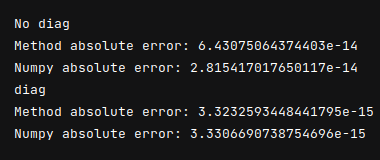
\includegraphics{images/res1.png}
\caption{Результат проверки работы метода на матрице размерности 10x10}
\label{fig:img1}
\end{figure}


Результат проверки работы метода на матрице размерности 100x100 представлен на рисунке~\ref{fig:img2}.


\begin{figure}[H]
\centering
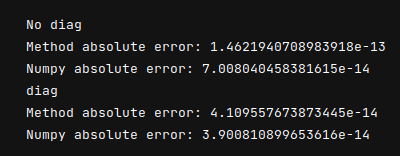
\includegraphics{images/res2.png}
\caption{Результат проверки работы метода на матрице размерности 100x100}
\label{fig:img2}
\end{figure}


Результат проверки работы метода на матрице размерности 300x300 представлен на рисунке~\ref{fig:img3}.

\begin{figure}[H]
\centering
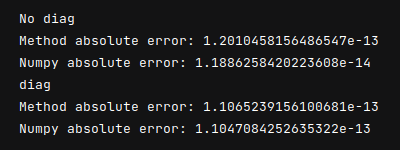
\includegraphics[width=0.8\textwidth]{images/res3.png}
\caption{Результат проверки работы метода на матрице размерности 300x300}
\label{fig:img3}
\end{figure}


\section{Выводы}
В результате выполнения лабораторной работы был реализован классический метод Гаусса, а также вспомогательные методы с генерацией матрицы с возможным диагональным преобладанием и тестированием работы метода.

Была проведена оценка абсолютной погрешности получившегося значения и было проведено сравнение с результатом работы библиотечного метода из библиотеки Numpy. Классический метод Гаусса показал менее точный результат на матрице без диагонального преобладания и примерно одинаковый результат на матрице с диагональным преобладанием.
\end{document}